\section{One hundred arms with AR(20): regret and PCS}
We evaluate the objective-specific policies on a $10\times10$ grid. The same deterministic two-peak mean surface is held fixed across configurations and noise replicates; the best-minus-second gap is $.20$, its norm is $3.807$, and its graph energy is $3.672$. Supplied bounds $B=6$, $S=3$ contain this truth. The mean regularizer is $H=.1I+.5L$ and the sensor variance is $.09$.

Innovation spatial correlation is the diagonally normalized resolvent $(I+3L)^{-1}$. Innovation scales are chosen so every marginal stationary deviation variance is one. Each arm has order 20. The configurations are:
\begin{itemize}
\item Persistent: $a_k$ proportional to $\exp(-k/6)$, with coefficient sum $.95$.
\item Weak: the same lag shape with coefficient sum $.35$.
\item Lag 20: $a_{20}=.85$ and the other coefficients are zero.
\item Heterogeneous: cyclic assignment of the persistent filter, a positive filter proportional to $\exp(-k/3)$ with sum $.65$, and alternating coefficients proportional to $(-1)^k\exp(-k/6)$ with absolute sum $.80$.
\item Independent shocks: the persistent filter with diagonal innovation covariance, retaining the same fixed mean surface and mean graph.
\end{itemize}
All filters are stable. Heterogeneous stationary cross-covariances use the pairwise companion Lyapunov equations; a separable covariance is not substituted.

There are 32 independent noise worlds per configuration, 1,000 calendar decisions per world, 14 learning rules, and four information benchmarks. Policies share the complete latent path and potential sensor readings within a world, but see only their selected reading after choosing. All learning rules initially measure each arm and then use square-age probes; round robin retains its strict cyclic schedule. The budget includes initial coverage. Gaussian policy draws use separate reproducible seeds. Practical UCB scale $.7$ and Thompson scale one are fixed across configurations.

Benchmarks always choose the true best-mean arm, greedily filter with known means and bandit readings, observe all past lag states, or observe all current rewards. The known-mean greedy filter is not an optimal causal policy. The past-state genie chooses the largest current conditional mean and lacks only fresh innovations. Known-mean benchmarks have artificial PCS one and are excluded from learning-policy PCS comparisons.

\begin{table}[p]
\centering\scriptsize
\begin{tabular}{llrrr}
\toprule
Dynamics & Policy & Oracle/$T$ & Mean/$T$ & PCS\\
\midrule
Persistent & IID UCB & 1.397 & 0.668 & 0.188\\
 & Independent AR UCB & 1.429 & 0.701 & 0.250\\
 & Joint mean UCB & 1.453 & 0.680 & 0.125\\
 & Joint predictive UCB & 1.426 & 0.715 & 0.125\\
 & Joint full-state UCB & 1.248 & 0.686 & 0.219\\
 & Joint predictive TS & 1.675 & 0.768 & 0.219\\
 & Contrast LUCB & 1.646 & 0.734 & 0.188\\
 & Top-two contrast TS & 2.064 & 0.809 & 0.250\\
\midrule
Weak & IID UCB & 2.131 & 0.607 & 0.719\\
 & Independent AR UCB & 1.890 & 0.367 & 0.656\\
 & Joint mean UCB & 1.994 & 0.487 & 0.812\\
 & Joint predictive UCB & 2.008 & 0.493 & 0.906\\
 & Joint full-state UCB & 1.838 & 0.321 & 0.531\\
 & Joint predictive TS & 2.160 & 0.608 & 0.719\\
 & Contrast LUCB & 2.088 & 0.570 & 0.844\\
 & Top-two contrast TS & 2.251 & 0.710 & 0.781\\
\midrule
Lag 20 & IID UCB & 2.160 & 0.622 & 0.531\\
 & Independent AR UCB & 1.841 & 0.545 & 0.656\\
 & Joint mean UCB & 1.943 & 0.427 & 0.688\\
 & Joint predictive UCB & 1.838 & 0.549 & 0.750\\
 & Joint full-state UCB & 1.760 & 0.534 & 0.688\\
 & Joint predictive TS & 2.230 & 0.773 & 0.562\\
 & Contrast LUCB & 2.025 & 0.502 & 0.844\\
 & Top-two contrast TS & 2.269 & 0.715 & 0.719\\
\midrule
Heterogeneous & IID UCB & 1.717 & 0.705 & 0.000\\
 & Independent AR UCB & 1.725 & 0.518 & 0.406\\
 & Joint mean UCB & 1.659 & 0.624 & 0.125\\
 & Joint predictive UCB & 1.617 & 0.700 & 0.250\\
 & Joint full-state UCB & 1.647 & 0.397 & 0.469\\
 & Joint predictive TS & 1.897 & 0.758 & 0.344\\
 & Contrast LUCB & 1.817 & 0.605 & 0.406\\
 & Top-two contrast TS & 2.211 & 0.751 & 0.562\\
\midrule
Independent shocks & IID UCB & 1.453 & 0.582 & 0.188\\
 & Independent AR UCB & 1.381 & 0.640 & 0.281\\
 & Joint mean UCB & 1.506 & 0.498 & 0.281\\
 & Joint predictive UCB & 1.491 & 0.633 & 0.375\\
 & Joint full-state UCB & 1.270 & 0.583 & 0.312\\
 & Joint predictive TS & 1.767 & 0.711 & 0.250\\
 & Contrast LUCB & 1.691 & 0.581 & 0.250\\
 & Top-two contrast TS & 2.151 & 0.724 & 0.375\\
\bottomrule
\end{tabular}

\caption{AR(20), 100 arms, budget 1,000, and 32 paired noise worlds per configuration. Oracle and permanent mean pseudo-regret are per decision; PCS targets the fixed best mean. Selected policies are shown; CSVs report all policies, Student-$t$ mean intervals, Wilson PCS intervals, actual best-mean-arm reward regret, MSE, and paired differences. Observed rankings are not simultaneous statistical claims.}
\label{tab:ar20}
\end{table}

\begin{figure}[p]
\centering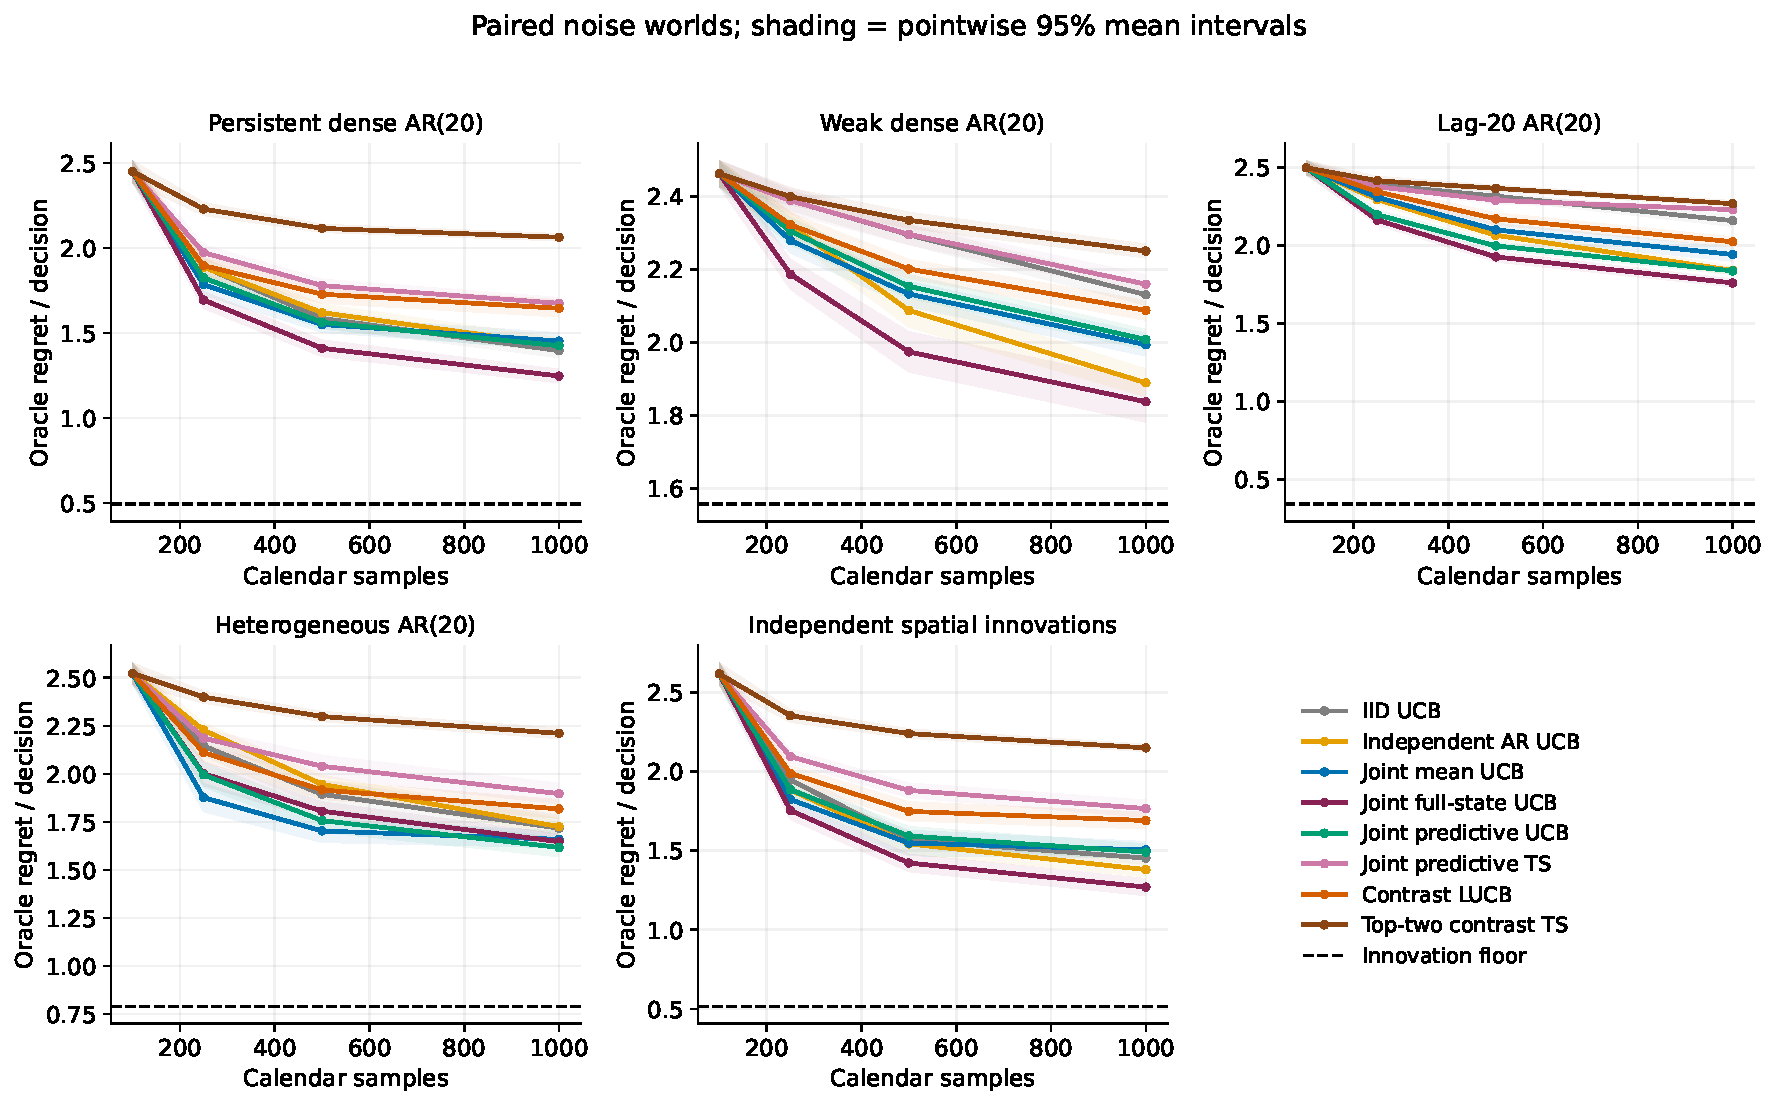
\includegraphics[width=\textwidth]{results/policies_ar20/oracle_regret.pdf}
\caption{Regret against the full-current-state oracle per decision. Dashed lines estimate the irreducible innovation coefficient. Shading gives pointwise 95\% intervals across independent worlds. The horizon includes 100 initial coverage observations.}
\label{fig:ar20-oracle}
\end{figure}
\begin{figure}[p]
\centering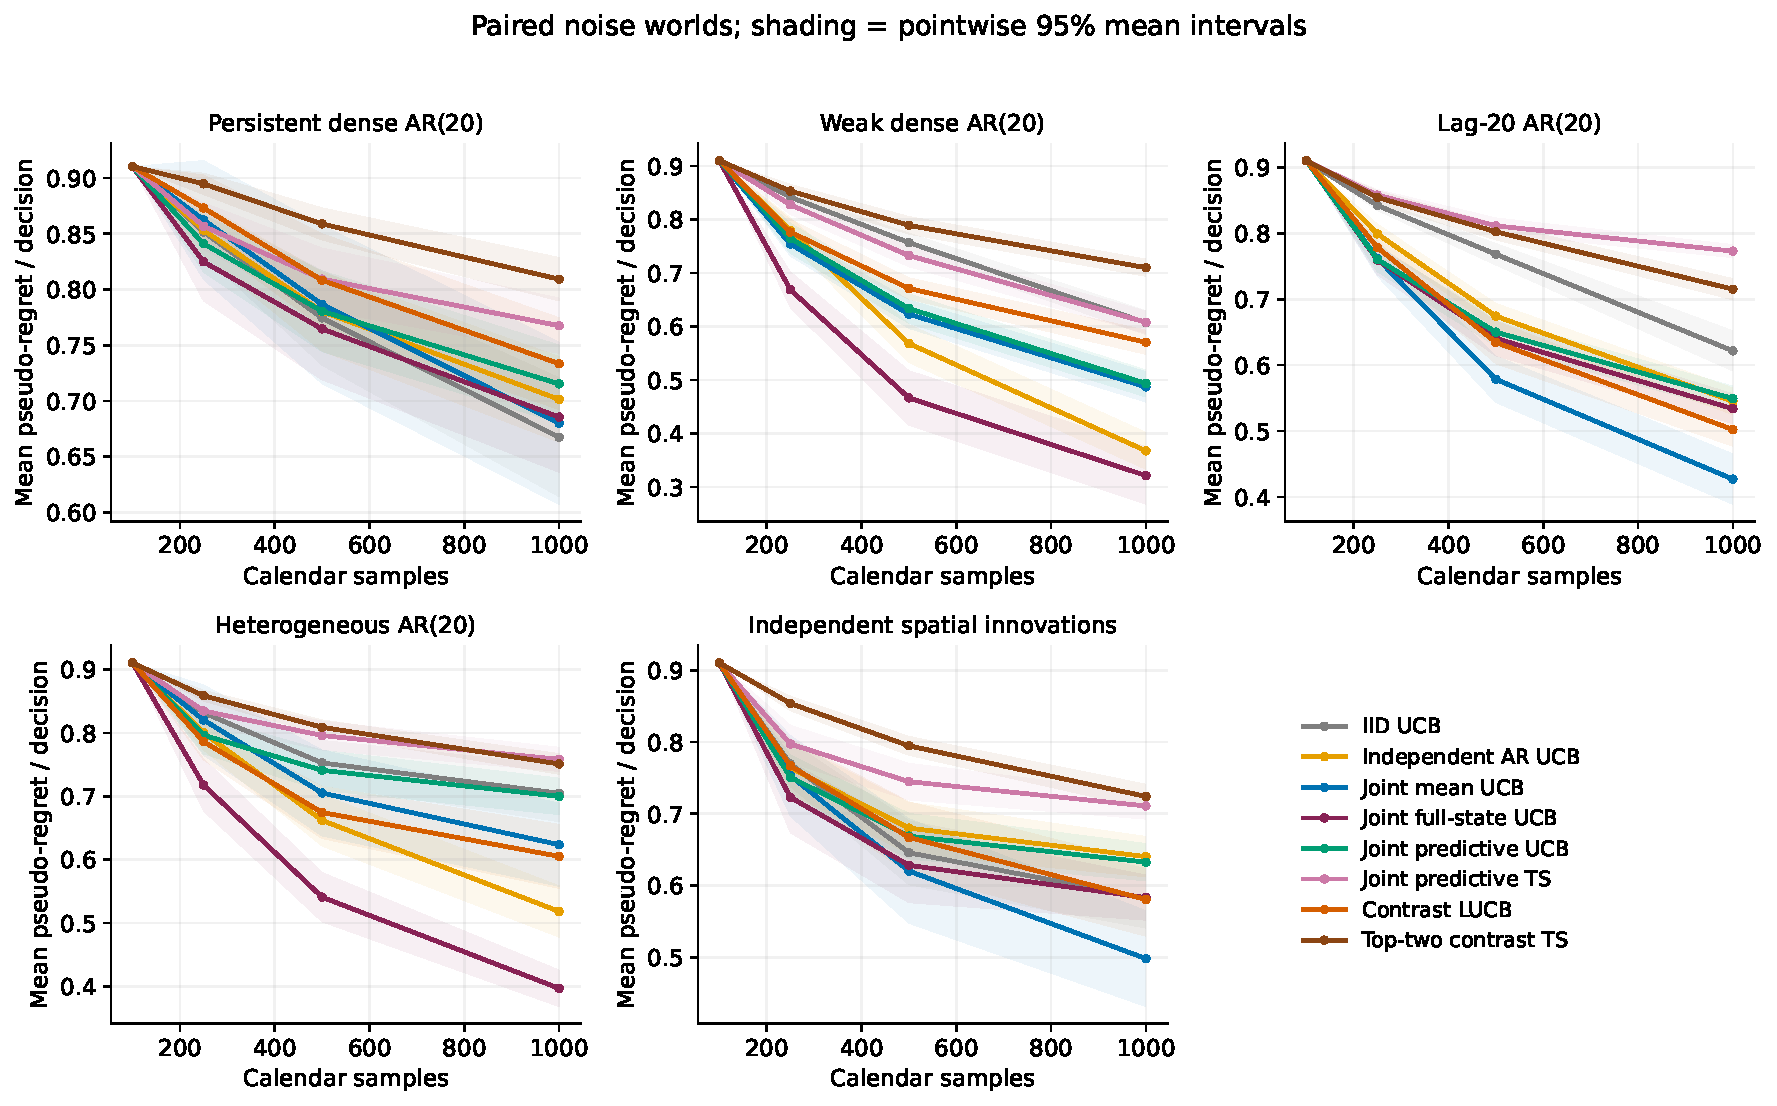
\includegraphics[width=\textwidth]{results/policies_ar20/mean_regret.pdf}
\caption{Permanent mean pseudo-regret per decision under the same paths. This comparator differs from both the current-state oracle and actual reward from the best permanent arm. Exploiting fluctuations can increase mean pseudo-regret while improving actual reward.}
\label{fig:ar20-mean}
\end{figure}
\begin{figure}[p]
\centering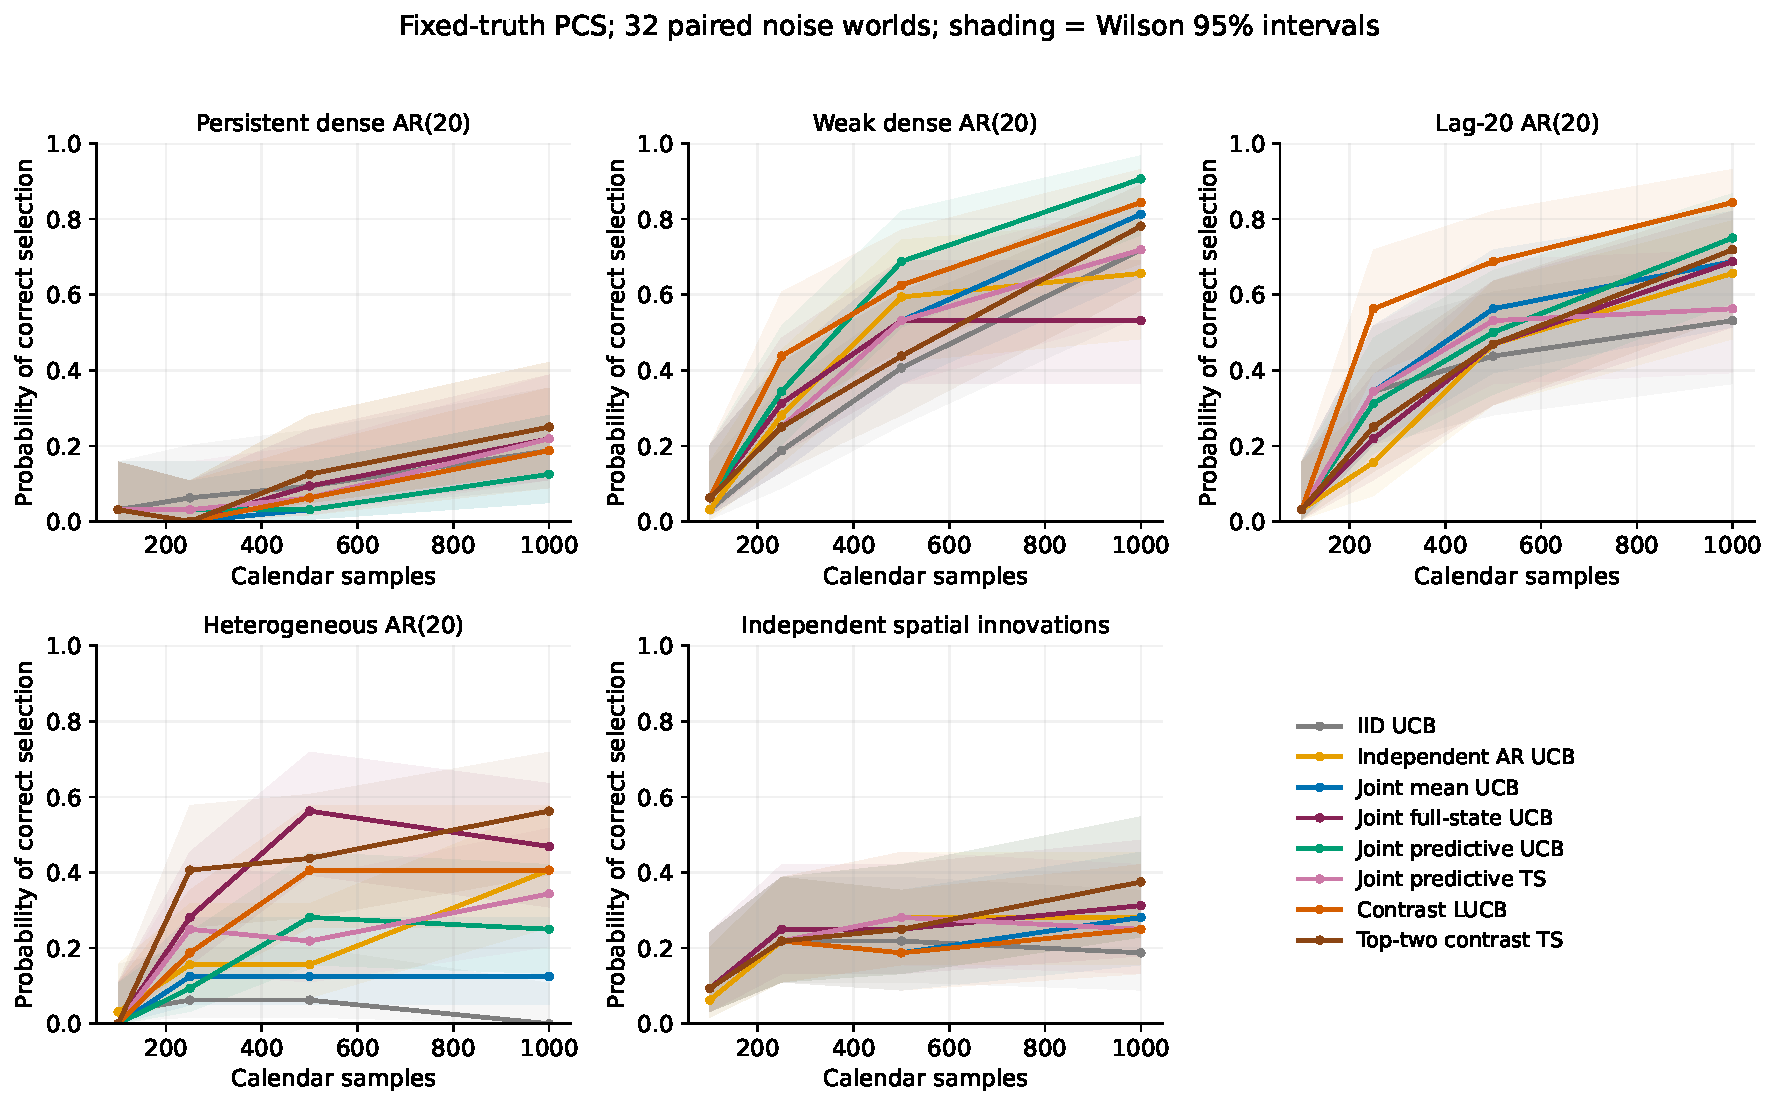
\includegraphics[width=\textwidth]{results/policies_ar20/pcs.pdf}
\caption{Fixed-truth PCS versus budget. Recommendations use permanent mean estimates. With 32 worlds, binomial uncertainty is substantial; Wilson intervals are reported in the CSV and findings. The fixed-budget decisions are not certified recommendations.}
\label{fig:ar20-pcs}
\end{figure}

The innovation-floor coefficients, estimated independently with 200,000 paired stationary Gaussian samples per configuration, are
Persistent $0.493$, Weak $1.556$, Lag 20 $0.340$, Heterogeneous $0.789$, Independent shocks $0.515$.

These are expectation bounds; a finite-world sampled regret need not exceed the estimated floor exactly. The full-past genie provides a separate path-simulation check. A declining finite-horizon regret ratio does not establish an asymptotic optimal coefficient.

For weak dependence, joint predictive UCB has PCS $0.906$, with Wilson interval $[0.758,0.968]$. The full-variance state UCB has smaller mean and oracle regret in this experiment. Selection accuracy and accumulated reward thus favor different decisions.

For lag-20 dependence, contrast LUCB gives PCS $0.844$ versus $0.281$ for round robin. The paired improvement is $0.562$ with approximate interval $[0.339,0.786]$. Joint mean UCB has smaller mean pseudo-regret, while full-state UCB has smaller oracle regret. The PCS-focused rule pays for comparison information rather than only extracting immediate reward.

For persistent dynamics, joint full-state UCB gives oracle regret $1.248$ per round versus $1.397$ for iid UCB. PCS remains poor, and joint mean UCB does not uniformly improve over iid UCB. Persistence helps state prediction while making permanent means harder to estimate. For a fully observed single arm, the long-run mean-noise scale is $q_i/(1-\sum_k a_{i,k})^2$; it is about 156 for the persistent profile. This full-observation scale illustrates the difficulty, without replacing the actual schedule-dependent likelihood.

For the same persistent state-UCB policy, mean pseudo-regret is $0.686$ per round, while actual reward regret against the stationary mean is $-0.308$ with interval $[-0.375,-0.240]$. The policy earns more than the best permanent mean by using predictable fluctuations, despite often choosing inferior permanent locations.

Removing fresh-innovation variance from Thompson draws improves oracle regret by 0.043--0.327 per round across these configurations. It does not uniformly improve the UCB rule. For homogeneous filters, adding a common positive variance inside a square root compresses differences between optimism bonuses; finite-budget performance also depends on exploration scale. These experiments compare fixed practical scales, not optimally tuned policy families.


The study validates computation and compares policies at one fixed mean surface. It does not establish general finite-budget optimality, robustness to incorrect graphs or unknown dynamics, or matching graph-dependent regret constants. The new implementation passes 588 assertions against dense likelihood and independent state calculations; large-model pilots exercise both 100-arm predictive policies. The analysis also checks paired-result completeness, nonnegative oracle/mean regret, and the pathwise identity $R_{\rm oracle}^{\pi}-R_{\rm oracle}^{b^*}=R_{\rm fixed}^{\pi}$.
